\section{Graphs}
\subsection{Introduction to Graphs}
Graphs are fundamental objects in discrete mathematics that model relationships between pairs of objects. Graphs arise in a wide array of disciplines but play an especially important role in computer science.

In an \bld{undirected graph}, the edges are unordered pairs of vertices, which is useful for modeling relationships that are symmetric. A graph consists of a pair of sets $(V,E)$, where $V$ is a set of vertices and $E$ is a set of edges. A graph is \bld{finite} if the vertex set is finite. A single element of $V$ is called a \bld{vertex} and is usually represented pictorially by label, or a dot with a label. Each edge in $E$ is a set of two vertices from $V$ and is drawn as a line connecting the two vertices.
\begin{center}
  \begin{tikzpicture}
    %VARIABLES
    \pgfmathsetmacro{\gsize}{1};
    \pgfmathsetmacro{\gnum}{5};

    \foreach[count=\i] \element in {a,b,c,d,e} { %domain
        \node (\element) at (\i * 360 / \gnum:\gsize) {$\element$};
        \node (\element-) at (\i * 360 / \gnum:\gsize + 0.5) {};
      }
    \foreach \j/\l in {a/b,a/c,b/c,b/e,c/d,d/e} { %a to b
        \draw (\j) -- (\l);
      }
    \node[anchor=east] (name) at (145:\gsize+.5) {An undirected graph}; %relation name
  \end{tikzpicture}
\end{center}
In the above graph, two edges cross each other, but there is no vertex at the crossing. The crossing is just a byproduct of how the graph is drawn on a two-dimensional surface. The graph above can be described by listing the vertex set and the edge set:
\begin{align*}
  V & = \{a,b,c,d,e\}                                       \\
  E & = \{\{a,b\},\{a,c\},\{b,c\},\{b,e\},\{c,d\},\{d,e\}\}
\end{align*}
A graph may appear to be disconnected into more than one piece but is still considered to be one graph. Here are two graphs, each with 5 vertices.
\begin{center}
  \begin{tikzpicture}
    %VARIABLES
    \pgfmathsetmacro{\gsize}{1};
    \pgfmathsetmacro{\gnum}{5};

    \foreach[count=\i] \element in {a,b,c,d,e} { %domain
        \node (\element) at (\i * 360 / \gnum:\gsize) {$\element$};
        \node (\element-) at (\i * 360 / \gnum:\gsize + 0.5) {};
      }
    \foreach \j/\l in {a/b,c/d,d/e} { %a to b
        \draw (\j) -- (\l);
      }
    \node[anchor=east] (name) at (145:\gsize+.5) {Graph $A$}; %relation name
  \end{tikzpicture}
  \begin{tikzpicture}
    %VARIABLES
    \pgfmathsetmacro{\gsize}{1};
    \pgfmathsetmacro{\gnum}{5};

    \foreach[count=\i] \element in {a,b,c,d,e} { %domain
        \node (\element) at (\i * 360 / \gnum:\gsize) {$\element$};
        \node (\element-) at (\i * 360 / \gnum:\gsize + 0.5) {};
      }
    \node[anchor=east] (name) at (145:\gsize+.5) {Graph $B$}; %relation name
  \end{tikzpicture}
\end{center}
\bld{Parallel edges} are multiple edges between the same pair of vertices. In defining graphs with parallel edges, it \itl{might} be important to have additional label besides the two endpoints to specify an edge in order to distinguish between different parallel edges. A graph can also have a \bld{self-loop} which is an edge between a vertex, and itself.
\begin{center}
  \begin{tikzpicture}
    %VARIABLES
    \pgfmathsetmacro{\gsize}{1};
    \pgfmathsetmacro{\gnum}{4};

    \foreach[count=\i] \element in {a,b,c,d} { %domain
        \node (\element) at (\i * 360 / \gnum:\gsize) {$\element$};
        \node (\element-) at (\i * 360 / \gnum:\gsize + 0.5) {};
      }
    \foreach \j/\l in {a/c,b/d,c/d} { %a to b
        \draw (\j) -- (\l);
      }
    \foreach \j/\l in {a/b} { %a to b TWICE (parallel edges)
        \draw (\j) to[bend left=20 / \gsize + 10] (\l);
        \draw (\l) to[bend left=20 / \gsize + 10] (\j);
      }
    \foreach \j in {c} { %a to a
        \draw (\j) to[bend left=65] (\j-)
        to[bend left=65] (\j);
      }
    \node[anchor=east] (name) at (145:\gsize+.5) {A graph with parallel edges and a self-loop}; %relation name
  \end{tikzpicture}
\end{center}
If a graph does not have parallel edges or self-loops, it is said to be a \bld{simple graph}.

\subsubsection*{Graph terminology}
\begin{center}
  \begin{tikzpicture}
    %VARIABLES
    \pgfmathsetmacro{\gsize}{1};
    \pgfmathsetmacro{\gnum}{5};

    \foreach[count=\i] \element in {a,b,c,d,e} { %domain
        \node (\element) at (\i * 360 / \gnum:\gsize) {$\element$};
        \node (\element-) at (\i * 360 / \gnum:\gsize + 0.5) {};
      }
    \foreach \j/\l in {a/b,a/c,b/c,b/e,c/d,d/e} { %a to b
        \draw (\j) -- (\l);
      }
    \node[anchor=east] (name) at (145:\gsize+.5) {Undirected graph example}; %relation name
  \end{tikzpicture}
\end{center}
\begin{itemize}
  \item If there is an edge between two vertices, they are said to be \bld{adjacent}. In the graph above, $d \tand e$ are adjacent, but $d \tand b$ are not adjacent.
  \item Vertices $b \tand e$ are the \bld{endpoints} of edge $\{b,e\}$. The edge $\{b,e\}$ is \bld{incident} to vertices $b tand e$.
  \item A vertex $c$ is a \bld{neighbor} of vertex $b$ if and only if $\{b,c\}$ is an edge. In the graph above, the neighbors of $b$ are the vertices $a,c, \tand e$.
  \item In a simple graph, the \bld{degree} of a vertex is the number of neighbors it has. In the graph above, the degree of $b$ is 3 and the degree of vertex $a$ is 2. The degree of vertex $b$ is denoted by $\deg(b)$.
  \item The \bld{total degree} of a graph is the sum of the degrees of all of the vertices. The total degree of the above graph is $2 + 3 + 3 + 2 + 2 = 12$.
  \item In a \bld{regular graph}, all the vertices have the same degree. In a \bld{$d$-regular graph}, all the vertices have degree $d$. The graph above is not regular because $\deg(a) \neq \deg(b)$. However, the graph below is 3-regular.
\end{itemize}
\begin{center}
  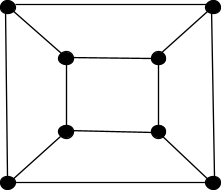
\includegraphics[width=.2\linewidth]{resources/3-regular graph.png}
\end{center}
\begin{itemize}
  \item A graph $H = (V_H,E_H)$ is a \bld{subgraph} of a graph $G = (V_G,E_G)$ if $V_H \subseteq V_G \tand E_H \subseteq E_G$. Note that any graph $G$ is a subgraph of itself.
\end{itemize}
\begin{center}
  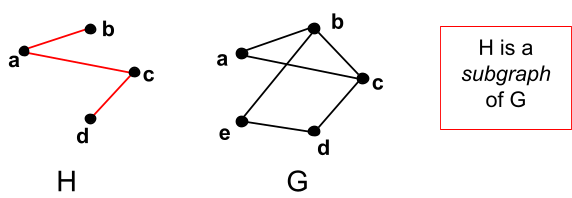
\includegraphics[width=.6\linewidth]{resources/H is a subgraph of G.png}
\end{center}

\subsubsection*{Theorem: Number of Edges and Total Degree}
Let $G = (V,E)$ be an undirected graph, simple or not. Then, twice the number of edges is equal to the total degree:
\[
  \sum_{v \in V} \deg(v) = 2 \cdot |E|
\]

\subsubsection*{Common Graphs}
Some graphs with special structure are given their own name and notation because they come up so frequently in graph theory.
\begin{center}
  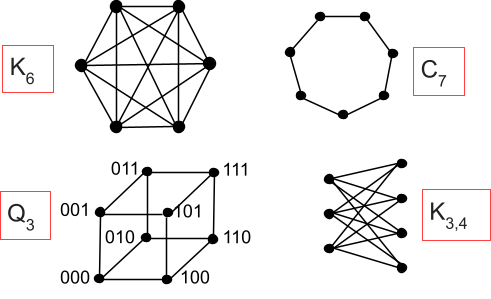
\includegraphics[width=0.6\linewidth]{resources/common graphs.png}
\end{center}
For the definition of all of these graphs, $n \in \bb{Z}^+$.
\begin{itemize}
  \item $K_n$ is called the \bld{complete graph} on $n$ vertices. $K_n$ has an edge between every pair of vertices. $K_n$ is sometimes called a \bld{clique} of size $n$ or an \bld{$n$-clique}.
  \item $C_n$ is called a cycle on $n$ vertices. The edges connect the vertices in a ring. Note that $C_n$ is well defined only for $n \geq 3$.
  \item The $n$-dimensional hypercube, denoted $Q_n$, has $2^n$ vertices. Each vertex is label with an $n$-bit string. Two vertices are connected by an edge if their corresponding labels differ only by one bit.
  \item $K_{n,m}$ has $n+m$ vertices, and $2nm$ edges. The vertices are divided into two sets: one with $m$ vertices and one set with $n$ vertices. There are no edges between vertices in the same set, but there is an edge between every vertex in one set and every vertex in the other set.
\end{itemize}

\subsection{Graph representations}
\begin{center}
  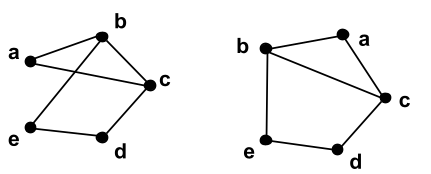
\includegraphics[width=0.5\linewidth]{resources/two similar graphs.png}
\end{center}
These two graphs look different, but that is only because they are drawn differently. The two graphs are actually the same graph because they have the same vertex and edge sets as shown below:
\begin{align*}
  V & = \{a,b,c,d,e\}                                       \\
  E & = \{\{a,b\},\{a,c\},\{b,c\},\{b,e\},\{c,d\},\{d,e\}\}
\end{align*}
The way a graph is drawn is not part of the graph itself.

\subsubsection*{Adjacency List Representation for Graphs}
In the \bld{adjacency list representation} of a graph, each vertex has a list of all its neighbors. Note that since the graph is undirected if vertex $a$ is in $b$'s list of neighbors, then $b$ must also be in $a$'s list of neighbors.

If a graph is represented using adjacency lists, the time required to list the neighbors of a vertex $v$ is proportional to $\deg(v)$, the number of vertices to be listed. In order to determine if $\{a,b\}$ is an edge, it is necessary to scan the list of $a$'s neighbors or the list of $b$'s neighbors. In the worst case, the time required is proportional to the larger of $\deg(a)$ or $\deg(b)$.

\subsubsection*{Matrix Representation for Graphs}
The \bld{matrix representation} for a graph with $n$ vertices is an $n \times n$ matrix whose entries are all either $0 \tor 1$, indicating whether or not each edge is present. The matrix representation of an undirected graph is symmetric.
\begin{center}
  \begin{tikzpicture}
    %VARIABLES
    \pgfmathsetmacro{\gsize}{1};
    \pgfmathsetmacro{\gnum}{5};

    \foreach[count=\i] \element in {a,b,c,d,e} { %domain
        \node (\element) at (\i * 360 / \gnum:\gsize) {$\element$};
        \node (\element-) at (\i * 360 / \gnum:\gsize + 0.5) {};
      }
    \foreach \j/\l in {a/b,a/c,b/c,b/e,c/d,d/e} { %a to b
        \draw (\j) -- (\l);
      }
    \node[anchor=east] (name) at (145:\gsize+.5) {}; %relation name
  \end{tikzpicture} $~~\Rightarrow~~$
  $
    \begin{bmatrix}
      0 & 1 & 1 & 0 & 0 \\
      1 & 0 & 1 & 0 & 1 \\
      1 & 1 & 0 & 1 & 0 \\
      0 & 0 & 1 & 0 & 1 \\
      0 & 1 & 0 & 1 & 0
    \end{bmatrix}
  $
\end{center}

\subsection{Graph isomorphism}
Two graphs are said to be \bld{isomorphic} if there is a correspondence between the vertex sets of each graph such that there is an edge between two vertices of one graph if and only if there is an edge between the corresponding vertices of the second graph. Essentially, the graphs are not identical but the vertices can be relabeled so that they are identical.

\subsubsection*{Definition of Isomorphic Graphs}
Let $G = (V,E) \tand G'=(V',E')$. $G \tand G'$ are isomorphic if there is a bijection $f: V \rightarrow V'$ such that for every pair of vertices $x,y \in V$, $\{x,y\} \in E$ if and only if $\{f(x), f(y)\} \in E'$. The function $f$ is called an \bld{isomorphism} from $G \tto G'$.

\begin{center}
  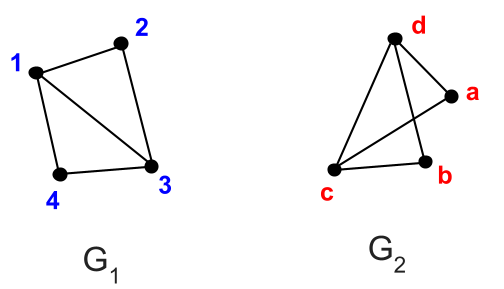
\includegraphics[width=0.4\linewidth]{resources/isomorphic graphs 1.png}
\end{center}
The following function is an isomorphism from the vertices of $G_1 \tto G_2$:
\[
  f(1) = d \qquad f(2) = a \qquad f(3) = c \qquad f(4) = b
\]

\subsubsection*{Theorem: Vertex Degree Preserved under Isomorphism}
Consider two graphs, $G \tand G'$. Let $f$ be an isomorphism from $G \tto G'$. For each vertex $v \tin G$, the degree of vertex $v \tin G$ is equal to the degree of vertex $f(v) \tin G'$.

\subsubsection*{}
The \bld{degree sequence} of a graph is a list of the degree of all of the vertices in non-increasing order.
\begin{center}
  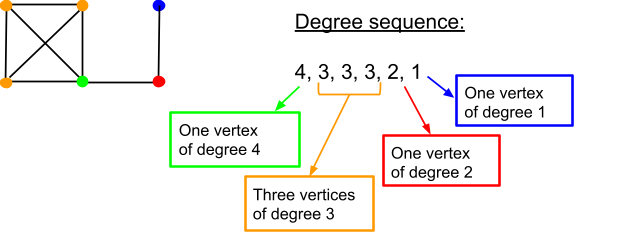
\includegraphics[width=0.7\linewidth]{resources/degree-sequence.png}
\end{center}

\subsubsection*{Theorem: Degree Sequence Preserved under Isomorphism}
The degree sequence of a graph is preserved under isomorphism.


\subsection{Walks, trails, circuits, paths, and cycles}
A \bld{walk} from $v_0 \tto v_l$ in an undirected graph $G$ is a sequence of alternating vertices and edges that starts and ends with a vertex:
\[
  \langle v_0,\{v_0,v_1\},v_1,\{v_1,v_2\},\ldots,v_{\ell-1},\{v_{\ell-1},v_\ell\},v_\ell\rangle
\]
Since the edges in a walk are completely determined by the vertices, a walk can also be denoted by the sequence of vertices:
\[
  \langle v_0,v_1,\ldots,v_\ell \rangle.
\]
However, keep in mind the sequence of vertices is a walk only if $\{v_{j-1},v_j\} \in E$ for each $j = 1,2,\ldots,\ell$. The \bld{length of a walk} is $\ell$, the number of edges in the walk. An \bld{open walk} is a walk in which the first and last vertices are not the same. A \bld{closed walk} is a walk in which the first and last vertices are the same.
\begin{itemize}
  \item A \bld{trail} is a walk in which no \itl{edge} occurs more than once.
  \item A \bld{path} is a walk in which no \itl{vertex} occurs more than once.
  \item A \bld{circuit} is a closed \itl{trail}.
  \item A \bld{cycle} is a \itl{circuit} is length at least 1 in which no vertex occurs more than once, except the first and last vertices which are the same.
\end{itemize}
Here are some examples of closed walks:
\begin{itemize}
  \item $\langle A,C,D,A \rangle$ is a \itl{trail}, a \itl{circuit}, and a \itl{cycle}.
  \item $\langle A,C,B,A,D,E,A \rangle$ is a \itl{trail} and a \itl{circuit}.
  \item $\langle A,B,A \rangle$ is \bld{not} a trail, circuit, or a cycle.
\end{itemize}
Since paths and cycles do not have any repeated edges, if a graph is simple, any cycle \itl{must} have length at least 3. The sequence $\langle v \rangle$ is not a cycle because a cycle, by definition, must have length at least 1. The sequence $\langle v,v \rangle$ is only a walk if there is a self-loop at vertex $v$.

\subsection{Graph connectivity}
Two vertices, $v \tand w$, are \bld{connected} if there is a path from $v \tto w$ (and thus also a path from $w \tto v$). A vertex is always considered to be connected to itself. The property of being connected can be extended to sets of vertices and the entire graph:
\begin{itemize}
  \item A set of vertices in a graph is said to be connected if every pair of vertices in the set is connected.
  \item A graph is said to be connected if every pair of vertices in the graph is connected, and is \bld{disconnected} otherwise.
\end{itemize}
A \bld{connected component} consists of a \itl{maximal} set of vertices that are connected as well as all the edges between two vertices in the set. A vertex that is not connected with any other vertex is called an \bld{isolated vertex} and is therefore a connected component with only one vertex.
\begin{center}
  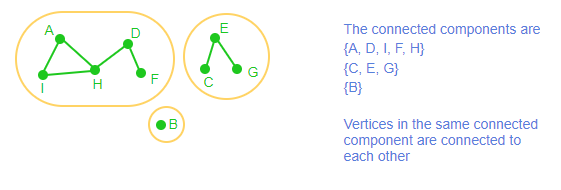
\includegraphics[width=0.6\linewidth]{resources/connected components example.png}
\end{center}

\subsubsection*{k-Connectivity}
In some networks, it is important to be able to guarantee connectivity, even if one or more vertices or edges are removed from a graph. The definition of connectivity can be extended to encompass resilience to vertex or edge failures.

\subsubsection*{Definition of a K-vertex-connected Graph}
An undirected graph $G$ is \bld{$k$-vertex-connected} if the graph contains at least $k + 1$ vertices and remains connected after any $k - 1$ vertices are removed from the graph. The \bld{vertex connectivity} of a graph is the largest $k$ such that the graph is $k$-vertex-connected. The vertex connectivity of a graph $G$ is denoted $\kappa(G)$.

The vertex connectivity of a graph is the minimum number of vertices whose removal disconnects the graph into more than one connected component.

When the graph is a complete graph, there is no set of vertices whose removal disconnects the graph. For the special case of $K_n$, the vertex connectivity $\kappa(K_n)$ is just defined to be $n - 1$.

\subsubsection*{Definition of a K-edge-connected Graph}
An undirected graph G is \bld{$k$-edge-connected} if removing any $k - 1$ or fewer edges results in a connected graph. The \bld{edge connectivity} of a graph is the largest $k$ such that the graph is $k$-edge-connected. The edge connectivity of a graph G is denoted $\lambda(G)$.

The edge connectivity of a graph is the minimum number of edges whose removal disconnects the graph into more than one connected component.

\subsubsection*{Theorem: Upper bound for Vertex and Edge Connectivity}
Let $G$ be an undirected graph. Denote the minimum degree of any vertex in $G$ by $\delta(G)$. Then,
\begin{align*}
  \kappa(G)  & \leq \delta(G)~~~\tand \\
  \lambda(G) & \leq \delta(G).
\end{align*}

\subsection{Euler circuits and trails}
An \bld{Euler circuit} is a circuit that contains every edge and every vertex. Note that a circuit, by definition, has no repeated edges, so an Euler circuit contains each edge exactly once.
\begin{center}
  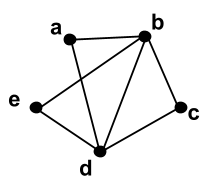
\includegraphics[width=0.2\linewidth]{resources/euler circuit example.png}
  Euler circuit: $\langle a,b,c,d,e,b,d,a \rangle$
\end{center}

\subsubsection*{Theorem: Characterization of Graphs that have an Euler Circuit}
An undirected graph $G$ has an Euler circuit if and only if $G$ is connected and every vertex in $G$ has even degree.
\[
  G~\text{has an Euler circuit}~\leftrightarrow G~\text{is connected and every vertex in $G$ has even degree}.
\]

\subsubsection*{Procedure to find a circuit in a Graph}
\begin{lstlisting}
Find a vertex w, that is not an isolated vertex.
Select any edge {w,x} incident to w.
(Since w is not isolated, there is always at least one such edge.)
Current trail T := <w,x>
last := x
While there is an edge {last, y} that has not been used in T:
  Add y to the end of T
  last := y
\end{lstlisting}

\subsubsection*{Procedure to find an Euler circuit in a Graph}
Use the procedure above to find any circuit in $G$. Call the circuit $C$. The algorithm continues to iterate the following steps until all the edges in $G$ are included in $C$:
\begin{enumerate}
  \item Remove all edges in $C$ from $G$. Remove any isolated vertices from $G$. Call the resulting graph $G'$.
  \item Find a vertex $w$ that is in $G' \tand C$.
  \item Find a circuit in $G'$ that begins and ends with $w$. Call the circuit $C'$.
  \item Combine circuit $C \tand C'$. Suppose $C$ starts and ends at vertex $v$. Create a new circuit that starts at $v$ and follows the edges in $C$ until $w$ is reached. The new circuit then follows the edges in $C'$ back to $w$ and then follows the rest of the edges in $C$ back to $v$. The new circuit is renamed $C$ for the next iteration.
\end{enumerate}


\subsubsection*{Euler trail}
An \bld{Euler trail} is an open trail that includes each edge. Note that a trail, by definition, has no repeated edges, so an Euler trail contains each edge exactly once. In an open trail, the first and last vertices are not equal.

\subsubsection*{Theorem: Characterizations of graphs that have an Euler trail}
An undirected graph $G$ has an Euler trail if and only if $G$ is connected and has exactly two vertices with odd degree. The Euler trail begins and ends with the vertices of odd degree.
\[
  G~\text{has an Euler trail}~\leftrightarrow G~\text{is connected and has exactly two vertices with odd degree}.
\]

\subsection{Hamiltonian cycles and paths}
A \bld{Hamiltonian cycle} in an undirected graph is a cycle that includes every vertex in the graph. Note that a cycle, by definition, has no repeated vertices or edges, except for the vertex which is at the beginning and end of the cycle. Therefore, every vertex in the graph appears exactly once in a Hamiltonian cycle, except for the vertex which is at the beginning and end of the cycle. A \bld{Hamiltonian path} in an undirected graph is a path that includes every vertex in the graph. Note that a path, by definition, has no repeated vertices or edges, so every vertex appears exactly once in a Hamiltonian path.

Note that a Hamiltonian cycle can be transformed into a Hamiltonian path by deleting the last vertex. Therefore if a graph has a Hamiltonian cycle, then the graph also has a Hamiltonian path.

Unlike Euler circuits and trails, there are no known conditions describing exactly which graphs have a Hamiltonian cycle or path. However, there are some cases in which a graph that does have a Hamiltonian cycle or path has a certain property.
\begin{itemize}
  \item Any graph that has a vertex with degree 1 does not have a Hamiltonian cycle.
  \item For $n \geq 3$, $K_n$ has a Hamiltonian cycle.
\end{itemize}

\subsection{Planar graphs}
Placing graphs on two-dimensional surfaces to avoid crossings is a classic problem in graph theory. The problem also arises in the field of graph drawing in which the goal is to draw complex graphs in a way that helps people visualize structure and patterns.

An \bld{embedding} for $G = (V,E)$ is an assignment of the vertices to points in the plane and an assignment of each edge to a continuous curve. The curve for each edge must start and edge at the two points corresponding to the endpoints of the edge. Essentially, an \itl{embedding is a way of drawing a graph} on a plane, because mathematically, a graph is just a set of vertices and a set of edges.

An embedding is said to be a \bld{planar embedding} if none of the edges cross. There is a crossing between two edges in an embedding if their curves intersect at a point that is not a common endpoint. An embedding of a graph can be planar or not planar, depending on whether it has a crossing. Planarity can also be defined as a property of the graph itself.

\subsubsection*{Definition of Planar Graphs}
A graph $G$ is a \bld{planar graph} if the graph has a planar embedding.

\begin{center}
  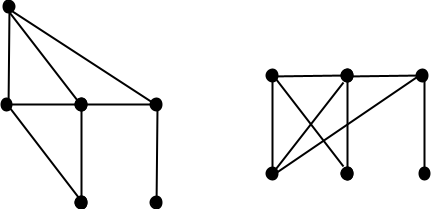
\includegraphics[width=0.4\linewidth]{resources/two embeddings.png}
\end{center}
\begin{itemize}
  \item The embedding on the left \itl{is planar}.
  \item The embedding on the right \itl{is \bld{not} planar}.
\end{itemize}

The \bld{complement of an embedding} is the set of all points in the plane that are not part of a curve corresponding to an edge. A planar embedding carves up the plane into continuous regions. A \bld{region} is a set of points in the complement of an embedding that forms a maximal continuous set, meaning that it is (continuous): possible to travel anywhere from any point in the region and (maximal): if any point were added to the region, it would no longer be continuous. In a planar embedding, there is always an infinite region called the \bld{exterior region}, which is region $V$ in the following graph.
\begin{center}
  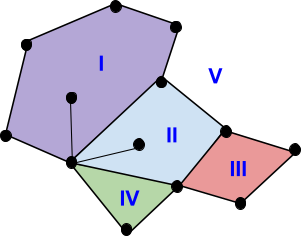
\includegraphics[width=0.4\linewidth]{resources/regions of a planar embedding.png}
\end{center}

\subsubsection*{Theorem: Euler's Identity for Regions in an Embedding}
Consider a planar embedding of a connected graph $G$. Let $v$ be the number of vertices in $G$, $e$ the number of edges, and $r$ the number of regions in the embedding. Then,
\[
  v - e + r = 2
\]

\subsubsection*{Degree of a Region}
\begin{center}
  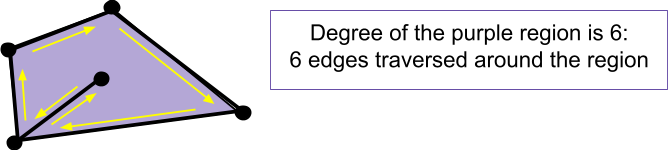
\includegraphics[width=0.6\linewidth]{resources/degree of a region.png}
\end{center}
Consider a planar embedding of a graph G. Think of a tiny bug walking all the way around the region along the edges of the graph. The degree of a region is the number of times the bug traverses an edge until it gets back to its starting location. Note that if an edge sticks out into a region, the edge can be traversed twice by the bug and therefore contributes 2 towards the degree of the region.

\subsubsection*{Theorem: Number of Edges in a Planar Graph}
Let G be a connected planar graph. Let $v$ be the number of vertices in G and $e$ the number of edges. If $v \geq 3$, then
\[
  e \leq 3v-6
\]

\subsection{Graph coloring}
Graph coloring is a classic problem in graph theory because it is useful in modeling resource constraints like scheduling.

\subsubsection*{Definition of Graph Coloring}
Let $G=(V,E)$ be an undirected graph and $C$ a finite set of colors. A \bld{valid coloring} of $G$ is a function $f: V \rightarrow C$ such that for every edge $\{x,y\} \in E, f(x) \neq f(y)$. If the size of the range of function $f$ is $k$, then $f$ is called a \bld{$k$-coloring} of $G$.

\subsubsection*{}
The coloring on the left is a valid coloring because no two adjacent vertices are assigned the same color. The coloring on the left is a 3-coloring because 3 colors are used. The coloring on the right is not a valid coloring because there is an edge whose endpoints are both colored pink.
\begin{center}
  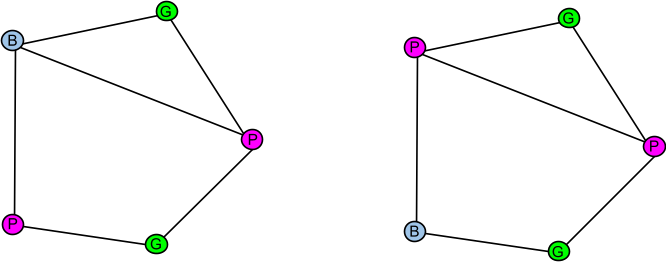
\includegraphics[width=0.5\linewidth]{resources/graph colorings.png}
\end{center}

\subsubsection*{Definition of the Chromatic Number of a Graph}
The \bld{chromatic number} of a graph $G$, denoted as $X(G)$ is the smallest $k$ such that there is a valid $k$-coloring of $G$. It is minimum number of colors that a graph requires to have a valid graph coloring.

\subsubsection*{}
In general, if $K_r$ is a subgraph of $G$, then there is a subset of $r$ vertices in $G$ such that every pair of vertices in the subset is connected by an edge. In any valid coloring of $G$, each of the $r$ vertices in the subset must be assigned a distinct color which implies that $X(G) \geq r$. The clique number of a graph G, denoted $\omega(G)$, is the largest $r$ such that $K_r$ is a subgraph of $G$.

\subsubsection*{Theorem: Relationship between the Clique Number of Chromatic Number}
If $G$ is an undirected graph, then
\[
  \omega(G) \leq X(g)
\]

\subsubsection*{Greedy coloring}
In general, it is difficult to determine the chromatic number of a graph $G$. However, there is an easy and natural method to color the vertices of a graph called the \itl{greedy coloring algorithm}. The \bld{greedy coloring algorithm} often leads to a color that uses a small number of colors, but there is no guarantee that it uses the \itl{smallest} number of colors possible for a given graph.

\subsubsection*{The Greedy Coloring Algorithm}
\begin{enumerate}
  \item Number the set of possible colors. Assume that there is a very large supply of different colors, even though they might not all be used.
  \item Order to vertices in any arbitrary order.
  \item Consider each vertex $v$ in order. Assign $v$ a color that is different from the color of $v$'s neighbors that have already been assigned that color. When selecting a color for $v$, use the lowest number color possible.
\end{enumerate}
The term "greedy" is used to describe a general paradigm for solving many different kinds of problems. Greedy algorithms typically solve a problem one piece at a time.

The greedy algorithm provides a way to upper bound the chromatic number of a graph.

\subsubsection*{Theorem: Upper bound for $X(G)$}
Let $G$ be an undirected graph. Let $\Delta(G)$ be the maximum degree of any vertex in $G$. Then,
\[
  X(G) \leq \Delta(G)+1
\]